%%% Template originaly created by Karol Kozioł (mail@karol-koziol.net) and modified for ShareLaTeX use

\documentclass[a4paper,11pt]{article}

\usepackage[T1]{fontenc}
\usepackage[utf8]{inputenc}
\usepackage{graphicx}
\usepackage{xcolor}

\renewcommand\familydefault{\sfdefault}
\usepackage{tgheros}
\usepackage[defaultmono]{droidmono}

\usepackage{amsmath,amssymb,amsthm,textcomp}
\usepackage{enumerate}
\usepackage{multicol}
\usepackage{tikz}
\usepackage{geometry}
\geometry{total={210mm,297mm},
left=25mm,right=25mm,%
bindingoffset=0mm, top=20mm,bottom=20mm}


\linespread{1.3}

\newcommand{\linia}{\rule{\linewidth}{0.5pt}}

% custom theorems if needed
\newtheoremstyle{mytheor}
    {1ex}{1ex}{\normalfont}{0pt}{\scshape}{.}{1ex}
    {{\thmname{#1 }}{\thmnumber{#2}}{\thmnote{ (#3)}}}

\theoremstyle{mytheor}
\newtheorem{defi}{Definition}

% my own titles
\makeatletter
\renewcommand{\maketitle}{
\begin{center}
\vspace{2ex}
{\huge \textsc{\@title}}
\vspace{1ex}
\\
\linia\\
\@author \hfill \@date
\vspace{4ex}
\end{center}
}
\makeatother
%%%

% custom footers and headers
\usepackage{fancyhdr}
\pagestyle{fancy}
\lhead{}
\chead{}
\rhead{}
\lfoot{Trabalho \textnumero{} 1}
\cfoot{}
\rfoot{Página \thepage}
\renewcommand{\headrulewidth}{0pt}
\renewcommand{\footrulewidth}{0pt}
%

% code listing settings
\usepackage{listings}
\lstset{
    language=Python,
    basicstyle=\ttfamily\small,
    aboveskip={1.0\baselineskip},
    belowskip={1.0\baselineskip},
    columns=fixed,
    breaklines=true,
    tabsize=4,
    prebreak=\raisebox{0ex}[0ex][0ex]{\ensuremath{\hookleftarrow}},
    frame=lines,
    showtabs=false,
    showspaces=false,
    showstringspaces=false,
    keywordstyle=\color[rgb]{0.627,0.126,0.941},
    commentstyle=\color[rgb]{0.133,0.545,0.133},
    stringstyle=\color[rgb]{01,0,0},
    numbers=left,
    numberstyle=\small,
    stepnumber=1,
    numbersep=10pt,
    captionpos=t,
    inputencoding=utf8,
    extendedchars=true,
    escapeinside={\%*}{*)}
}

\usepackage{seqsplit}
\usepackage{wrapfig}
\usepackage{graphicx}
\graphicspath{ {images/} }

%%%----------%%%----------%%%----------%%%----------%%%

\begin{document}

\title{Trabalho Individual sobre protocolo Diffie-Hellman-Merkle}

\author{Fernando Paladini, Segurança em Computação (INE5429)}

\date{04/10/2016}

\maketitle

\section*{1) O protocolo Diffie-Hellman-Merkle e alguns exemplos}

O protocolo de acordo de chaves \textit{Diffie-Hellman} (ou \textit{Diffie-Hellman-Merkle}) é um protocolo seguro para realizar a troca (ou acordo) de chaves criptográficas em um canal público. É um dos protocolos mais utilizados no mundo e também um dos primeiros de chave pública, definido por Ralph Merkle, Whitfield Diffie e Martin Hellman em 1976. 
\newline\newline
\noindent \textbf{Uma descrição intuitiva para o protocolo de acordo de chaves Diffie-Hellman-Merkle (DHM) segue logo abaixo:}

\begin{wrapfigure}{l}{0.5\textwidth}
    \centering
    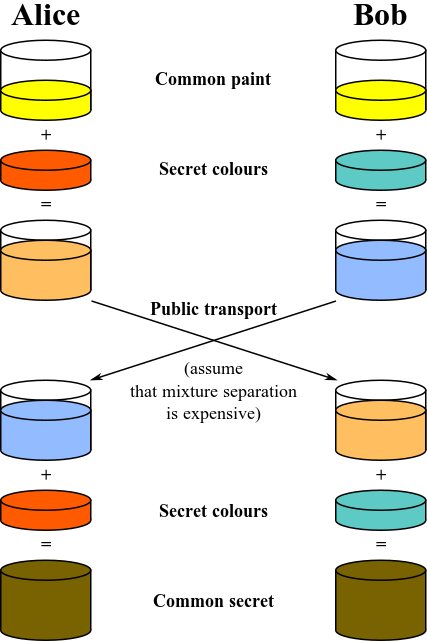
\includegraphics[width=0.5\textwidth]{intuitivo}
\end{wrapfigure}

\noindent Na imagem ao lado, os números muito grandes utilizados pelo DHM foram substituídos por cores para fazer a explicação intuitiva do protocolo. O processo começa com duas partes, que vamos chamar de Alice e Bob, acordando uma cor que não precisa ser mantida em segredo, mas deve ser trocada a cada novo acordo de chaves. No nosso exemplo, a cor é o amarelo. Alice e Bob então devem escolher uma cor cada um e essa cor deve ser mantida privada - vermelho e ciano, respectivamente. Uma das partes cruciais do protocolo vem agora, quando Alice e Bob devem \textit{misturar} a sua "cor privada" com a "cor pública", acordada mutuamente pelas partes. Essa \textit{mistura} resulta na cor laranja para Alice e na cor azul para Bob. Após isso, Alice e Bob trocam as cores (pode ser realizado de forma pública) e então \textit{misturam} a cor recebida da outra parte com a sua cor privada. Para ilustrar, no nosso exemplo Alice deve misturar azul com o vermelho e Bob deve misturar laranja com ciano. O resultado final é uma cor que será idêntica tanto para Alice quanto para Bob, ou seja, o segredo em comum entre Alice e Bob.
\newline\newline
\noindent \textbf{Uma descrição mais técnica do DHM segue abaixo:}

\noindent A implementação original do DHM utiliza o grupo multiplicativo dos inteiros módulo \textit{p}, onde \textit{p} é um número primo e \textit{g} é uma raiz primitiva módulo \textit{p}. O objetivo desta artimanha é que a chave secreta resultante pode ser qualquer valor entre 1 e \textit{p-1}. 

O processo começa com as duas partes envolvidas, que vamos chamar de Alice e Bob, escolhendo um módulo \textit{p} e uma base \textit{g} comum. Após acordar esses dois valores, as partes devem escolher um número inteiro \textbf{secreto} e cada um deve gerar um valor $g^{q} \pmod{p}$, onde \textit{q} é o inteiro secreto escolhido por cada parte. Para ilustrar, vamos supor que Alice escolha um inteiro secreto 8, enquanto que Bob escolhe um inteiro secreto 16. Então Alice (A) e Bob (B) devem gerar os seguintes valores:
\begin{align*}
A = g^{8} \pmod{p} \\
B = g^{16} \pmod{p}
\end{align*}

\noindent Agora Alice e Bob devem trocar os valores gerados. De forma simplificada:
\begin{align*}
Alice \overset{A}{\longrightarrow} Bob \\
Alice \overset{B}{\longleftarrow} Bob
\end{align*}

Finalmente, para calcular a chave secreta (\textit{s}), Alice deve calcular $s = B^{a} \pmod{p}$ e Bob deve calcular $s = A^{b} \pmod{p}$. Agora Alice e Bob podem utilizar essa chave secreta compartilhada como uma chave de encriptação que é conhecida apenas por eles, permitindo-os enviar mensagens sobre um canal de comunicação aberto mas de forma privada. Note que boa parte dos valores (\textit{p}, \textit{g}, $g^{a} \pmod{p}$ e $g^{b} \pmod{p}$) foram enviados de forma pública, enquanto que os valores \textit{a}, \textit{b} e $g^{ab} \pmod{p} = g^{ba} \pmod{p}$ são secretos. Note também que para fazer um exemplo que seja realmente seguro os valores de \textit{a}, \textit{b} e \textit{p} teriam que ser extremamente maiores, possuindo números com centenas de dígitos.

Para exemplificar o protocolo com um número um pouco maior, vamos utilizar o número primo $p = 773$ e a sua raiz primitiva $g = 730$. O número privado de Alice será $a = 128$ e o de Bob será $b = 64$.  Denotaremos o segredo compartilhamento novamente como $s$.
\noindent \begin{align*}
A = g^{a} \pmod{p} = 730^{128} \pmod{773} = 560 \\
B = g^{b} \pmod{p} = 730^{64} \pmod{773} = 670 \\
s = B^{a} \pmod{p} = 670^{128} \pmod{773} = 441 = 560^{64} \pmod{p} = A^{b} \pmod{p}
\end{align*}

Dessa forma, Alice e Bob agora possuem um segredo compartilhado que pode ser usado como chave para algum algoritmo de encriptação para que as duas partes possam então se comunicar em um canal público de forma segura. Nota: para realizar os cálculos mostrados de forma simplificada acima, um interpretador de Python versão 2.7.12 foi utilizado.

Os códigos, desenvolvidos em Python e testados na sua versão 2.7.12 está disponível logo abaixo:

\begin{lstlisting}[caption=Arquivo dhm.py.]
#!/usr/bin/env python
# -*- coding: utf-8 -*-

'''
Classe responsavel por representar uma parte interessada dentro do algoritmo de acordo de chaves Diffie-Hellman-Merkle (DHM).
'''

import random

class DHM(object):

	def __init__(self, p, g):
		self.private = random.getrandbits(512)
		self.p = p
		self.g = g

	def public_key(self):
		'''
		Gera a "chave publica" do DHM. Supondo que a parte em questao seja Alice, este metodo vai 
		gerar o valor que sera trocado publicamente com Bob.
		
		Returns:
			g^{a} \pmod{p} = g**a mod p

		'''
		return pow(self.g, self.private, self.p)

	def shared_secret_key(self, key):
		'''
		Gera o segredo compartilhado do DHM a partir da chave recebida. Supondo que a parte em questao
		seja Alice, este metodo vai gerar o segredo compartilhado entre Alice e Bob, parte fianl do
		protocolo DHM.

		Args:
			key: a chave publica da outra parte interessada.

		Returns:
			key^{a} \pmod{p} = key**a mod p
		'''
		return pow(key, self.private, self.p)
\end{lstlisting}

\begin{lstlisting}[caption=Arquivo dhm\_utils.py.]
#!/usr/bin/env python
# -*- coding: utf-8 -*-

from random import randrange
from fractions import gcd
import sys

class DHMUtils(object):

    @staticmethod
    def num_coprimos(n):
        '''
        Funcao que calcula o totiente de Euler de n (ou o numero de coprimos de 'n').
        '''
        num_coprimos = 0
        for i in range(n):
            if (gcd(i, n) == 1):
                num_coprimos += 1
        return num_coprimos

    @staticmethod
    def fatores_primos(n):
        '''
        Funcao que calcula todos os fatores primos de 'n' (ate que a sua raiz quadrada seja atingida).
        Retorna uma lista ordenada dos fatores primos de 'n'.
        '''
        fatores = set()
        i = 2
        while (i**2 <= n):
            if (n % i == 0):
                n = n // i
                fatores.add(i)
            else:
                i += 1
        fatores.add(n)
        return sorted(fatores)

    @staticmethod
    def raiz_primitiva(n):
        '''
        Funcao que encontra uma raiz primitiva de um inteiro n dado.
        '''
        p = DHMUtils.num_coprimos(n)
        fatores = DHMUtils.fatores_primos(p)
        while (True):
            a = randrange(1, n)
            if (all(pow(a, p // f, n) != 1 for f in fatores)):
                return a
\end{lstlisting}

\begin{lstlisting}[caption=Arquivo lcg.py.]
#!/usr/bin/env python3
# -*- coding: utf-8 -*-

import sys
import time

"""

Esta classe gera numeros pseudo-aleatorios utilizando o algoritmo LCG (Linear Congruential Generator).
Para chamar esta classe a partir da linha de comando basta digitar:
    
    $ python lcg.py <qtd_de_bits>

Onde "<qtd_de_bits>" eh a quantidade de bits que o numero gerado deve possuir. Exemplo:

    $ python lcg.py 32
    [LCG] Gerando numero de 32 bits...
    [LCG] Numero: 4174021489

Referencias:
    https://en.wikipedia.org/wiki/Linear_congruential_generator
    https://en.wikipedia.org/wiki/Combined_Linear_Congruential_Generator
    http://www.eternallyconfuzzled.com/tuts/algorithms/jsw_tut_rand.aspx
    https://rosettacode.org/wiki/Linear_congruential_generator

"""
class lcg(object):

    def __init__(self, seed = int(time.time()), m = 2**32, a = 1664525, c = 1013904223, size = None):
        """
            O construtor da classe do gerador de numeros pseudo-aleatorios eh altamente customizavel e
            recebe alguns parametros com valores padrao baseados no livro "Numerical Recipes: The Art 
            of Scientific Computing" (Press, WH; Teukolsky, SA; Vetterling, WT; Flannery, BP).

            Por padrao vai gerar um numero de 32 bits, mas caso um "size" seja fornecido, vai gerar
            somente numeros com "size" bits.

            Args:
                seed: valor de semente para iniciar o gerador de numeros pseudo-aleatorios. Se nao 
                      informado, utiliza o Unix Timestamp (Epoch) de acordo com as informacoes do sistema.
                m: o modulo, cujo valor padrao eh 2^32 / 4294967296.
                a: o multiplicador, cujo valor padrao eh 1664525.
                c: o incremento, cujo valor eh 1013904223.
                size: o tamanho em bits do numero a ser gerado, cujo valor padrao eh None (na prática eh 32).

            Returns:
                Esse metodo não retorna nada.
                
        """
        self.a = a
        self.c = c
        self.seed = seed
        self.size = size
        if self.size:
            self.m = 2**size
        else:
            self.m = m

    def rand(self):
        """
        Gera um numero aleatorio utilizando o algoritmo LCG, que eh descrito pela relacao
        de recorrencia expressa a seguir:

            Xn+1 = (a * Xn + c) mod m

        Onde: 
            m: o modulo (0 < m)
            a: o multiplicador (0 < a < m)
            c: o incremento (0 <= c < m)
            X: sequencia de valores pseudo-aleatorios.
            X0: o "seed" ou valor de começo.
            Xn+1: o proximo numero a ser gerado.

        Se uma instancia dessa classe possuir o atributo "size" definido no momento da construcao do objeto
        ou definido posteriormente em uma chamada ao metodo seed(self, new_seed), entao o numero gerado de 
        forma pseudo-aleatoria possuira "size" bits (ficara dentro de um loop enquanto nao atingir essa 
        quantidade de bits estipulada). Caso a instancia nao possua o atributo "size" definido, entao o
        numero pseudo-aleatorio gerado possuira ate 32 bits.

        Args:
            Este metodo nao recebe nenhum argumento.

        Returns:
            Um valor numerico pseudo-aleatorio de "size" bits.

        """
        self.seed = self.seed * self.a + self.c
        num = self.seed % self.m
        if self.size:
            while (num.bit_length() < self.size):
                self.seed = self.seed * self.a + self.c
                num = self.seed % self.m
        return num

    def randint(self, a, b):
        """
        Gera um numero aleatorio que esta entre os intervalos "a" e "b". 

        O numero a ser gerado, denominado "num", será maior ou igual a "a" e menor ou igual
        a "b". Em outras palavras, a <= num <= b.

        Args:
            a: valor numerico de limite inferior para o numero a ser gerado.
            b: valor numerico de limite superior para o numero a ser gerado.

        Returns:
            Um valor numerico pseudo-aleatorio que esta entre os valores a e b.

        """
        self.seed = self.seed * self.a + self.c
        num = self.seed % self.m
        while (not (a <= num <= b)):
            self.seed = self.seed * self.a + self.c
            num = self.seed % self.m
        return num

    def seed(self, new_seed):
        """
        Metodo para mudar o valor do seed para algum valor desejado.

        Args:
            new_seed: um valor numerico para indicar o novo valor de seed.

        Returns:
            Esse método não retorna nada.

        """
        self.seed = new_seed

    def size(self, new_size):
        """
        Metodo para mudar a quantidade de bits que o numero gerado terA.

        Args:
            new_size: um valor numerico para indicar a nova quantidade de bits do numero gerado.

        Returns:
            Esse metodo não retorna nada.

        """
        if self.size != new_size:
            self.size = new_size
            self.m = 2**new_size

 
if (__name__ == "__main__"):
    
    bits = int(sys.argv[1])

    print("[LCG] Gerando número de {} bits...".format(bits))
    print("[LCG] Número: {}".format(lcg(size=bits).rand()))
\end{lstlisting}

\begin{lstlisting}[caption=Arquivo primality.py.]
#!/usr/bin/env python3
# -*- coding: utf-8 -*-

import sys
import time
from lcg import lcg

"""

As classes deste arquivo verificam se os numeros fornecidos sao primos e geram numeros 
primos de tamanho variavel de bits de forma pseudo-aleatoria.

Para executar esse arquivo a partir da linha de comando basta digitar:
    
    $ python primality.py <qtd_de_bits>

Onde "<qtd_de_bits>" eh a quantidade de bits que o numero gerado deve possuir. Exemplo:

    $ python primality.py 128
    [MillerRabin] Procurando primo...
    [MillerRabin] 304159568226184448912103696911866306307 é primo!
    [Fermat] Procurando primo...
    [Fermat] 301970148924118150955226359108149582211 é primo!

Referencias:
    https://en.wikipedia.org/wiki/Fermat%27s_little_theorem
    https://en.wikipedia.org/wiki/Pseudoprime
    https://pt.wikipedia.org/wiki/Teste_de_primalidade_de_Miller-Rabin
    https://en.wikipedia.org/wiki/Miller%E2%80%93Rabin_primality_test
    https://pt.wikipedia.org/wiki/Teste_de_primalidade_de_Fermat
    https://jeremykun.com/2013/06/16/miller-rabin-primality-test/
    http://mathworld.wolfram.com/Rabin-MillerStrongPseudoprimeTest.html
    https://www.youtube.com/watch?v=qfgYfyyBRcY

"""
class MillerRabin(object):

    @staticmethod
    def verificar_testemunha(possivel_testemunha, p, exp, resto):
        """
        Verifica se a possivel testemunha de que um numero nao eh primo eh
        realmente testemunha. Se for, significa que o numero que esta 
        sendo testado tem uma testemunha da sua nao primalidade, de forma
        que a hipotese de que o numero testado eh primo pode ser descartada.

        Args:
            possivel_testemunha: a possivel testemunha de que "p" nao eh primo.
                                 Sera testemunha caso a^d ≢ 1 (mod n) e 
                                 a^((2^r)d) ≢ -1 (mod n) para todo 0 <= r <= s - 1.
            p: o numero para o qual a primalidade esta sendo testada.
            exp, resto: numeros inteiros, onde 'resto' eh um numero impar.

        Returns:
            True se a possivel testemunha for uma testemunha de que "p" nao eh primo.
            False se a possivel testemunha nao for uma testemunha de verdade.

        """
        possivel_testemunha = pow(possivel_testemunha, resto, p)
        if ((possivel_testemunha == 1) or (possivel_testemunha == p - 1)):
            return False

        for _ in range(exp):
            possivel_testemunha = pow(possivel_testemunha, 2, p)
            if (possivel_testemunha == (p - 1)):
                return False

        return True
    
    @staticmethod
    def verificar_primalidade(p, certeza=100):
        """
        O teste de Miller-Rabin eh um importantissimo teste probabilistico da primitividade de um numero dado.
        Se um numero passa nesse teste significa que ele tem uma probabilidade >= 75% de ser um numero primo,
        mas ate este numero ser provado como sendo um numero primo ele eh considerado apenas um "pseudoprimo".

        Ao aplicar o mesmo teste varias vezes, a margem de erro pode ser diminuida aleatoriamente, de forma
        que a margem de erro final seja consideravelmente baixa. Ele eh baseado no "Pequeno Teorema de Fermat",
        que consiste do "Teste de primalidade de Fermat".

        Args:
            p: o numero a ser testado.
            certeza: o grau de "certeza" de que este numero seja de fato um numero primo. Valor padrao eh 100, o
                     que significa que o teste sera aplicado 100 vezes.

        Returns:
            True se o numero eh um (pseudo-)primo.
            False se o numero nao eh primo.

        """
        if (p == 2 or p == 3): 
            return True
        elif (p < 2): 
            return False

        resto = p - 1
        exp = 0
        while (resto % 2 == 0):
            resto = resto/2
            exp += 1

        for _ in range(certeza):
            possivel_testemunha = lcg().randint(2, p - 2)
            if (MillerRabin.verificar_testemunha(possivel_testemunha, p, exp, resto)):
                return False

        return True

    @staticmethod
    def encontrar_primo(bits=None):
        """
        Encontra um numero primo que possui 'bits' bits utilizando uma busca com numeros gerados de forma pseudo-aleatoria. 

        Args:
            bits: quantidade de bits que o numero primo deve possuir. Se nenhum valor for informado, sera usado 32 bits.
        
        Returns:
            Um valor numerico com 'bits' bits e que eh primo.

        """
        bits = bits or 32
        random = lcg(size=bits)

        while (True):
            primo = random.rand()
            if (MillerRabin.verificar_primalidade(primo)):
                return primo

class FermatPrimality(object):

    @staticmethod
    def verificar_primalidade(p):
        """
        Verifica se o numero dado 'p' eh um numero primo atraves do metodo de Fermat, tambem conhecido 
        como "Teste de Primalidade de Fermat". Este eh um dos metodos mais simples para verificar se um 
        numero eh primo ou não (e provavelmente um dos mais elegantes também). Neste metodo a composicao
        do numero dado eh verificada e os numeros que falham no teste nao sao primos.

        Esta implementação nao leva em consideracao os numeros de Carmichael, que sao infinitos e
        passam pelo teste, mas nao são primos. Portanto, a partir deste teste podemos obter apenas
        numeros que sao considerados "pseudoprimos".

        Args:
            p: o numero que sera testado a primalidade.

        Returns:
            True significa que o numero eh pseudoprimo, ou seja, provavelmente eh primo (existem falso-positivos).
            False significa que o numero eh composto, ou seja, nao eh primo.

        """
        if (p == 2):
            return True
        if (not p & 1):
            return False

        if (pow(2, p-1, p) == 1):
            return True
        else:
            return False

    @staticmethod
    def encontrar_primo(bits=None):
        """
        Encontra um numero primo que possui 'bits' bits utilizando uma busca com numeros gerados de forma pseudo-aleatoria. 

        Args:
            bits: quantidade de bits que o numero primo deve possuir. Se nenhum valor for informado, sera usado 32 bits.
        
        Returns:
            Um valor numerico com 'bits' bits e que eh primo.

        """
        bits = bits or 32
        random = lcg(size=bits)

        while (True):
            primo = random.rand()
            if (FermatPrimality.verificar_primalidade(primo)):
                return primo

if (__name__ == "__main__"):

    bits = int(sys.argv[1])

    print("[MillerRabin] Procurando primo...")
    print("[MillerRabin] {} eh primo!".format(MillerRabin.encontrar_primo(bits)))

    time.sleep(2)
    
    print("[Fermat] Procurando primo...")
    print("[Fermat] {} eh primo!".format(FermatPrimality.encontrar_primo(bits)))
\end{lstlisting}

\begin{lstlisting}[caption=Arquivo key_exchange.py.]
#!/usr/bin/env python
# -*- coding: utf-8 -*-

'''
Implementa um exemplo do protocolo Diffie-Hellman-Merkle (DHM).
'''

from random import randrange
from fractions import gcd
from dhm import DHM
from dhm_utils import DHMUtils
from primality import MillerRabin

# Procurando primo de 512 bits (possuem mais do que 100 digitos)
prime = MillerRabin.encontrar_primo(30)

# Procurando raizes primitivas desse número primo e obtendo alguma de forma aleatória.
primitive_root = DHMUtils.raiz_primitiva(prime)

# Calculando chave pública de Alice e Bob
alice = DHM(prime, primitive_root)
bob = DHM(prime, primitive_root)
A = alice.public_key()
B = bob.public_key()

# Calculando segredo compartilhado
secretAlice = alice.shared_secret_key(B)
secretBob = bob.shared_secret_key(A)

print("Quantidade de dígitos do número primo: {}".format(len(str(prime))))
print("O segredo compartilhado entre Alice e Bob é igual?")
print(secretAlice == secretBob)
\end{lstlisting}

\noindent As execuções só foram possíveis com números primos com cerca de 20~30 dígitos. Ao tentar utilizar números primos com muito mais dígitos que isso (por volta de 100, por exemplo), o computador ficava processando por muito tempo e nos 10 minutos em que aguardei uma resposta, nada foi obtido. O processo foi extremamente lento ao tentar encontrar uma raiz primitiva do número primo dado, que também consumia muita memória. As execuções, realizadas com primos que variavam de 20~30 dígitos, resultaram no seguinte:

\begin{lstlisting}
$ python key_exchange.py 
Quantidade de digitos do numero primo: 24
O segredo compartilhado entre Alice e Bob eh igual?
True
$ python key_exchange.py 
Quantidade de digitos do numero primo: 25
O segredo compartilhado entre Alice e Bob eh igual?
True
\end{lstlisting}

\section*{3) Ataque Man in the middle}

Um ataque \textit{man in the middle} pode ser realizado no protocolo de acordo de chaves Diffie-Hellman-Merkle quando uma entidade monitora (secretamente) a comunicação entre duas partes interessadas em estabelecer um acordo de chaves utilizando DHM e altera as mensagens entre elas. Como o protocolo original não possui autenticação, ele torna-se vulnerável a esse tipo de ataque. Caso o atacante, que vamos chamar de Carl, consiga obter as chaves parciais \textit{A} e \textit{B} de Alice e Bob, então é possível que ele crie uma chave secreta com cada um deles e simule a troca de mensagens direta caso o canal não seja seguro o suficiente.

Para solucionar o problema de \textit{man in the middle}, pode-se utilizar o protocolo de acordo de chaves Diffie-Hellman-Merkle numa versão autenticada que utiliza certificados de chave pública. A ideia é mais ou menos a seguinte: antes de Alice e Bob executarem o protocolo DHM, cada um obtêm um par de chaves (pública e privada) e também um certificado para a chave pública. Durante a execução do protocolo, Alice assina algumas mensagens, como por exemplo o valor $g^{a} \pmod{p}$. Bob faz exatamente a mesma coisa. Mesmo que um invasor Carl possa interceptar as mensagens entre Alice e Bob, ele não pode falsificar as assinaturas de Bob e Alice sem suas respectivas chaves privadas. Um protocolo DHM melhorado com a utilização de certificados de chave púbica pode resolver o problema de \textit{Man in the middle} existente no algoritmo original.

\section*{4) Protocolo sem raíz primitiva}

Se \textit{g} não for uma raiz primitiva mod \textit{p}, então \textit{p} gerará apenas um subgrupo do grupo multiplicativo $\mathbb{Z}/ p \mathbb{Z}$. Dessa forma, a segurança do protocolo de acordo de chaves Diffie-Hellman-Merkle será \textbf{proporcional} à ordem de \textit{g} em $\mathbb{Z}/ p \mathbb{Z}$, quando a ordem ideal é (obviamente) a ordem total do grupo. Assim, um número muito grande (suficientemente grande) precisa ser escolhido para que a ordem do subgrupo seja afetada, chegando a um nível plausível de segurança.

\end{document}
